\chapter{Xu hướng tấn công ứng dụng web hiện nay và hướng phát triển ứng dụng webfuzzer}
\section{Xu hướng tấn công ứng dụng web hiện nay}
Bảo mật luôn là vấn đề hàng đầu trong nhiều lĩnh vực khác nhau của cuộc sống, đặc biệt trong lĩnh vực phần mềm máy tính/di động và ứng dụng web trong thời đại cách mạng công nghiệp 4.0 hiện nay. Những ứng dụng quan trọng liên quan đến tài chính, thông tin cá nhân của người dùng cũng đang được cung cấp rộng rãi bởi các ngân hàng, ví điện tử, mạng xã hội,... Tất cả điều đó hấp dẫn rất nhiều tin tặc và tổ chức tội phạm mạng, dẫn đến nguy cơ bị tấn công của các phần mềm nói chung và các ứng dụng web nói riêng. Đối với ứng dụng web, ngoài việc khai thác các lỗ hổng bảo mật ở tầng mạng như tấn công từ chối dịch vụ (denial of service - \acrshort{dos}), các phương pháp giả mạo bộ nhớ đệm (\acrshort{dns}/HTTP web server cache poisoning), chiếm tên miền phụ (subdomain takeover),..., tầng ứng dụng (sẽ được trình bày ở \textbf{Chương 3}) thì việc tấn công các ứng dụng web được \textbf{lưu trữ ảo} (virtual hosting) và khai thác những \textbf{lỗ hổng 0-day và n-day mới} của các công cụ, khung thức do bên thứ ba cung cấp cho ứng dụng web đang trở thành xu hướng. \par
Hiện nay, việc khai thác các lỗ hổng bảo mật trên một ứng dụng web còn có thể ảnh hưởng đến nhiều ứng dụng web khác thông qua sự phổ biến của các dịch vụ lưu trữ ảo. Lưu trữ ảo là một phương pháp cho phép lưu trữ (hosting) nhiều tên miền ứng dụng web trên một máy chủ vật lý. Việc sử dụng hosting ảo giúp tiết kiệm chi phí vận hành, tiết kiệm quỹ địa chỉ IPv4 sẵn có cũng như tạo điều kiện cho các dịch vụ hosting phát triển mạnh mẽ, cho phép họ dễ dàng cung cấp dịch vụ, quản lý việc hosting nhiều ứng dụng web khác nhau trên cùng một máy chủ vật lý, không cần phải đầu tư nhiều về phần cứng lẫn băng thông. Những máy chủ web thường dùng để triển khai hosting ảo là \textbf{Nginx}, \textbf{Apache}, hoạt động tốt trên các phiên bản của hai hệ điều hành máy chủ phổ biến nhất hiện nay là \textbf{Ubuntu Server} và \textbf{Windows Server}. Hai máy chủ web này lưu giữ mã nguồn và nội dung của các ứng dụng web trong quá trình vận hành dưới dạng các thư mục con (đối với \textbf{Apache}) hoặc các khối máy chủ (Nginx server block - đối với \textbf{Nginx}) tương ứng với các ứng dụng web riêng biệt, đồng thời cung cấp nhiều tính năng quản lý hosting, cải thiện hiệu năng, đảm bảo bảo mật cho các ứng dụng web trong cụm hosting ảo. Các tính năng trên thường xuyên được cải tiến, nâng cấp và bản thân \textbf{Apache} cũng như \textbf{Nginx} có chương trình trả thưởng cho các lỗ hổng bảo mật của họ (bug bounty program) rất hậu hĩnh, chúng ta có thể tạm yên tâm về khía cạnh bảo mật của các máy chủ web này nếu được cấú hình chuẩn bởi nhà cung cấp dịch vụ. Tuy nhiên việc sử dụng hosting ảo cũng tồn tại một số nhược điểm.
\begin{itemize}
    \item Sự tập trung nhiều ứng dụng web lại một chỗ gây ra rủi ro sụp đổ tại một điểm (single point failure). Khi có sự cố về phần cứng máy chủ web hoặc một ứng dụng web trong cụm bị tấn công từ chối dịch vụ, khả năng đáp ứng người dùng của những ứng dụng web khác sử dụng chung dịch vụ hosting ảo cũng sẽ bị ảnh hưởng, do sử dụng chung máy chủ vật lý và băng thông. 
    \item Các rủi ro bảo mật cho các ứng dụng web dùng chung hosting chủ yếu đến từ chính các ứng dụng web trong cụm chứ không từ máy chủ web như \textbf{Nginx} hay \textbf{Apache}, và việc đảm bảo bảo mật cho mỗi ứng dụng web tham gia hosting chung phải do chính chủ sở hữu của từng ứng dụng web trực tiếp quản lý. Tuy dịch vụ hosting ảo có thể hỗ trợ việc này một phần, thông qua một số tính năng/bộ lọc giúp kiểm soát, giới hạn quyền truy cập, bảo mật cook/ies cũng như sao lưu và phục hồi dữ liệu của \textbf{Nginx} và \textbf{Apache}, nhưng về mặt lý thuyết, một ứng dụng web trong cụm hosting ảo bị thoả hiệp (compromised) sẽ đồng nghĩa với việc tất cả các ứng dụng web còn lại đều bị thỏa hiệp. Điều này có được là do tin tặc hoàn toàn có khả năng truy xuất nội dung (bên trong các thư mục con, khối máy chủ trong hệ thống) và can thiệp vào các dịch vụ vận hành của các ứng dụng web khác.
\end{itemize}
Hiện nay, các dịch vụ tường lửa ứng dụng web (web application firewalls - \acrshort{waf}) ngày càng hoàn thiện cùng với nhiều cách hiện thực tốt nhất (best practices) được thống nhất trong cộng đồng lập trình viên, áp dụng rộng rãi trong chính bản thân nhiều ngôn ngữ lập trình và khung thức, công cụ nhằm chống lại việc khai thác những lỗ hổng bảo mật thường gặp của ứng dụng web (như \acrshort{dos}, \acrshort{sqli}, \acrshort{xss}, remote code execution - \acrshort{rce},...). Một vài ví dụ tiêu biểu có thể kể đến như các dịch vụ tường lửa \textbf{ModSecurity}, \textbf{CloudFlare}, \textbf{Citrix}, \textbf{AppTrana},..., các thư viện mã hóa và làm sạch dữ liệu đầu vào (input sanitizer) trên các ngôn ngữ lập trình phổ biến như PHP (HTML Purifier \parencite{htmlpurifier}, PHP Intrusion Detection System, PHP Password Lib, PHPSecLib), NodeJS (awesome-nodejs-security, thư viện Helmet của express framework), ReactJS (dompurify, xss, xss-filters), ESAPI \parencite{esapi}, AntiXSS \parencite{antiXSS},... Trong bối cảnh đó, một trong những hướng tấn công đáng để thử cho những tin tặc là điều tra và khai thác các ứng dụng web có lỗi trong những cụm hosting ảo này. Việc này tuy có thể mất nhiều thời gian công sức hơn tìm và khai thác các lỗ hổng bảo mật trên ứng dụng web mục tiêu của ta nhưng nếu thành công thì hậu quả để lại khó có thể đong đếm được do có rất nhiều trang web của những tổ chức lớn đang sử dụng dịch vụ hosting ảo. Và thông thường, những ứng dụng web quan trọng của một tổ chức nào đó (ví dụ như \href{https://bkpay.hcmut.edu.vn/bkpay/home.action}{BKPay} hay \href{https://mybk.hcmut.edu.vn/stinfo/}{ứng dụng quản lý} điểm số, thông tin cá nhân của sinh viên và cán bộ công nhân viên trong trường,...) thường sẽ được hosting chung để tiện trong công tác quản lý, nâng cấp, bảo mật và bảo trì thường xuyên. Giả sử như một ứng dụng web có lỗ hổng bảo mật và bị khai thác thì các ứng dụng web quan trọng khác cũng chung hosting sẽ ngay lập tức có nguy cơ cực kì cao sẽ bị thỏa hiệp, dẫn đến những mất mát to lớn về tài chính, về sự vận hành của cả tổ chức cũng như lộ thông tin cá nhân của rất nhiều người. \par
Một hướng tấn công đặc biệt hiệu quả hiện nay là khai thác những lỗ hổng bảo mật 0-day và n-day. Lỗ hổng 0-day là các lỗ hổng bảo mật trên phần mềm, phần cứng hoặc firmware mà nhà cung cấp các sản phẩm này chưa biết để vá lỗi. Thuật ngữ 0-day có thể được hiểu là chính bản thân lỗ hổng hoặc những cuộc tấn công đầu tiên sử dụng lỗ hổng đó. Sau khi một cuộc tấn công 0-day đã được công khai, lỗ hổng được nhà cung cấp thừa nhận và đang tiến hành vá lỗi, các tin tặc có thể viết mã khai thác để tấn công các hệ thống/ứng dụng sử dụng các sản phẩm chưa được vá lỗi đó. Thuật ngữ 1-day hay n-day dùng để chỉ ra thời gian (số ngày) giữa lúc cuộc tấn công diễn ra so với thời điểm nhà cung cấp công bố lỗ hổng hoặc để ám chỉ những lỗ hổng 0-day đã biết nhưng chưa có mã khai thác trên những môi trường khác nhau (ví dụ lỗ hổng A đã được khai thác thành công trên trình duyệt web Firefox trên hệ điều hành Windows nhưng chưa có mã khai thác lỗi A trên Ubuntu hay Android). Trách nhiệm của nhà cung cấp là công bố lỗ hổng ngay sau thời gian quy định (ví dụ như 90 ngày sau khi lỗ hổng được báo cáo đối với Project Google Zero) hoặc ngay khi có bản vá lỗi để cảnh báo các cá nhân và doanh nghiệp đang sử dụng sản phẩm của mình có động thái cập nhật bản vá hoặc tự vệ nếu lỗ hổng vẫn chưa được vá. Đồng thời các nhà cung cấp cùng các nhà phân phối và quản trị viên dưới quyền có trách nhiệm to lớn phải vá lỗ hổng n-day đó càng nhanh càng tốt để giảm thiểu thiệt hại không đáng có cho người dùng. Khái niệm lỗ hổng bảo mật và phơi bày thông tin thường gặp (common vulnerabilities and exposures - \acrshort{cve}) và liệt kê điểm yếu thường gặp của phần mềm (common weakness enumuration - \acrshort{cwe}) cũng được hình thành từ quá trình phát hiện - tấn công - vá lỗi liên tục này. \acrshort{cve} là một danh sách các lỗ hổng bảo mật được đặt mã hiệu và định danh của từng lỗ hổng kèm theo ít nhất một tài liệu tham khảo liên quan về lỗ hổng đó đã được công bố công khai. Danh sách này cũng như trang web tra cứu các \acrshort{cve} \parencite{CVE-details} và \acrshort{cwe} \parencite{CWE-details} được duy trì để phục vụ cho cộng đồng bởi \href{http://cve.mitre.org/}{MITRE Corporation}. Mục đích của CVE là để hệ thống các lỗ hổng, thuận tiện cho việc chia sẻ thông tin cũng như điều tra về các lỗ hổng có liên quan trong quá khứ của một nhà cung cấp nào đó. \par
Lỗ hổng bảo mật 0-day có thể xuất hiện ở bất cứ phần mềm, hệ thống, công cụ, khung thức nào, từ phía người dùng lẫn phía máy chủ ứng dụng web. Những lỗ hổng lớn gây nhiều thiệt hại thường nằm ở các trình duyệt web phổ biến như Google Chrome, Firefox, Safari; các khung thức và hệ quản trị nội dung (content management system - \acrshort{cms}) như Telerik, WordPress, Joomla, Wix, Shopify,...; các máy chủ web và dịch vụ lưu trữ, điện toán đám mây như Nginx, Apache, Microsoft Azure, Amazon Web Service,... Bằng việc sử dụng các lỗ hổng n-day hoặc các \acrshort{cve} liên quan đên các sản phẩm trên, tin tặc có thể tổ chức tấn công hàng loạt các cá nhân/doanh nghiệp sử dụng các sản phẩm đó với phiên bản thích hợp, chưa cập nhật bản vá. Khả năng thành công của dạng tấn công này gần như là tuyệt đối trong trường hợp sản phẩm đang được vận hành có cùng phiên bản và môi trường mà sản phẩm đó đang chạy trên, dẫn đến những vụ lộ thông tin cá nhân, thay đổi giao diện (deface), chiếm tên miền phụ,... của một số lượng cực lớn các trang web. Tiêu biểu có thể kể đến một loạt 3 \acrshort{cve} rất nguy hiểm của Telerik Web UI \parencite{telerik-CVEs} trong năm 2017 cho phép tin tặc tải lên bất kì tệp độc hại nào cũng như tự do thực thi mã trên các ứng dụng web sử dụng các phiên bản Teleril Web UI cũ, hay 10 \acrshort{cve} của Wordpress \parencite{wordpress-CVEs} trong năm 2019 thông qua việc khai thác lỗ hổng \acrshort{xss} và \acrshort{rce}.\par
Hai hướng tấn công phổ biến đã trình bày ở trên ngày càng tỏ ra hiệu quả và phổ biến hiện nay, một trong những điểm chung của hai cách thức trên là rất khó để có thể tự động hóa bởi công cụ. Không như các phương pháp quét hoặc thử sai khác, việc điều tra hosting ảo cũng như viết mã khai thác các \acrshort{cve} trên nhiều môi trường khác nhau phải được thực hiện bằng tay. Một điểm chung nữa là việc tấn công các ứng dụng web kém bảo mật trong cụm hosting ảo cũng như việc hình thành các \acrshort{cve} phần lớn đều bắt nguồn từ các lỗ hổng bảo mật ở tầng ứng dụng (đã được trình bày ở \textbf{Chương 3}) rồi được tổng quát hóa, định danh và phân loại theo dạng lỗ hổng và nhà cung câp sản phẩm tương ứng. Các lỗ hổng đó là cơ sở cho sự xuất hiện của rất nhiều vấn đề về bảo mật trên ứng dụng web, đồng thời các những phương pháp tự động hóa trong việc kiểm thử các lỗ hổng đó cũng đã có sẵn và ngày càng được hoàn thiện hơn bởi sự đóng góp của cộng đồng. Từ hai điểm chung và những phân tích trên, chúng tôi nhận thấy một trong những hướng hiệu quả và cấp thiết để hiện thực công cụ kiểm thử các ứng dụng web theo đề tài luận văn là tập trung phát hiện các lỗ hổng bảo mật ở tầng ứng dụng với khả năng tự động hóa càng cao càng tốt.
\section{Phạm vi và hướng phát triển ứng dụng webfuzzer}
Trong phạm vi luận văn tốt nghiệp này, tôi sẽ áp dụng phương pháp kiểm thử fuzzing dưới dạng kiểm thử hộp đen để hiện thực công cụ \textbf{webfuzzer}. Ngoài khả năng tự động hóa cao, việc áp dụng phương pháp này sẽ đem lại nhiều lợi ích khác.
\begin{itemize}
    \item Linh hoạt trong việc kiểm thử nhiều ứng dụng web sử dụng các công nghệ, mô hình, khung thức phát triển phần mềm khác nhau, cũng như cho phép kiểm thử số lượng lớn ứng dụng web trong một khoảng thời gian ngắn.
    \item Đơn giản hóa và chuẩn hóa việc kiểm thử các lỗ hổng bảo mật trên những ứng dụng web có thiết kế cao cấp và phức tạp. Những ứng dụng này thường có số lượng dòng code có thể lên đến hàng nghìn thậm chí hàng triệu dòng, việc kiểm thử mã nguồn đối với phương pháp hộp trắng hoặc hộp xám sẽ khó khăn hơn nhiều.
    \item Dễ dàng đạt được khả năng tự động hóa cao so với việc quét mã nguồn của ứng dụng. Nhìn chung quá trình phát triển công cụ bằng phương pháp này không yêu cầu kĩ năng lập trình cao hoặc những kĩ thuật nhận diện lỗ hổng quá đặc thù.
    \item Chủ yếu tập trung vào việc kiểm thử chức năng của ứng dụng, không quan tâm đến giao diện, hiệu năng hay trải nghiệm người dùng. Điều này giúp ta có mục tiêu rõ ràng và tiết kiệm công sức cho quá trình thiết kế, cải tiến các trường hợp kiểm thử. 
\end{itemize}
Tương tự như trong lĩnh vực kiểm thử phần mềm, việc áp dụng phương pháp kiểm thử fuzzing dưới dạng kiểm thử hộp đen trong quá trình kiểm thử bảo mật ứng dụng web cũng sẽ có một số hạn chế như sau.
\begin{itemize}
    \item Do không nắm được mã nguồn của ứng dụng web nên chiến thuật tốt nhất là ta chỉ nên tập trung kiểm tra những chỗ thường phát sinh lỗ hổng nhất, hoặc "đoán mò" và vượt qua (bypass) cách thức phòng thủ của ứng dụng bằng việc thử sai và làm rối (tampering) dữ liệu kiểm thử.
    \item Số lượng trường hợp kiểm thử kết hợp với các kĩ thuật bypass đã biết là quá lớn, yêu cầu nhiều kinh nghiệm thực tế của người lập trình để chọn lọc và viết ra được một công cụ nhanh và ổn định, tối ưu hóa tài nguyên máy tính và thời gian thực thi. Ta buộc phải đánh đổi thời gian và tài nguyên đó hoặc chấp nhận kiểm thử trên một tập dữ liệu nhỏ hơn chỉ chứa những trường hợp thường gặp nhất.
    \item Phải có hiểu biết sâu rộng về các lỗ hổng bảo mật, đồng thời thường xuyên cập nhật các trường hợp kiểm thử và kĩ thuật tấn công/phòng thủ mới để bổ sung vào công cụ.
\end{itemize}
Hơn nữa, vấn đề đạo đức nghề nghiệp phải luôn luôn được đặt lên trên hết. Trước và trong quá trình kiểm thử ta phải có thỏa thuận với nhà cung cấp ứng dụng web về mục đích và cách thức tiến hành của mình, hoặc, xác định rõ động cơ của bản thân là để phát hiện những lỗ hổng nguy hiểm và sẽ báo cáo lại với nhà cung cấp để họ vá lỗi, tăng cường bảo mật và bảo vệ quyền lợi của người dùng ứng dụng đó. Bên cạnh đó ta cũng cần phải lưu ý về vấn đề pháp lý của mỗi vùng lãnh thổ địa lý hoặc quy định của những nhà cung cấp khác nhau, cũng như trang bị một số hiểu biết nhất định để bảo vệ danh tính và sự riêng tư của bản thân khi tiến hành kiểm thử số lượng lớn các ứng dụng web xuyên quốc gia.\par
Trong quá trình tìm hiểu và so sánh giữa các phương pháp, công cụ kiểm thử bảo mật ứng dụng web hiện tại, chúng tôi nhận thấy sử dụng chức năng \texttt{Intruder} của Burp Suite là phương pháp phù hợp nhất để tự động hóa quá trình phát hiện các lỗ hổng bảo mật ở tầng ứng dụng của các ứng dụng web thông qua thông điệp \acrshort{http}. \texttt{Intruder} là chức năng triển khai tấn công ứng dụng web tự động, mạnh mẽ và dễ cấu hình. Chức năng này có thể được sử dụng thực hiện những cuộc tấn công với phạm vi trải dài từ đơn giản tới phức tạp, từ vét cạn (brute-force) mật khẩu, thư mục ứng dụng web đến phát hiện các lỗ hổng bảo mật web ở tầng ứng dụng bằng phương pháp fuzzing. Hình \ref{fig:send-base-request-1} sau mô tả giao diện chính của chức năng này.
\begin{figure}[H]
    \centering
        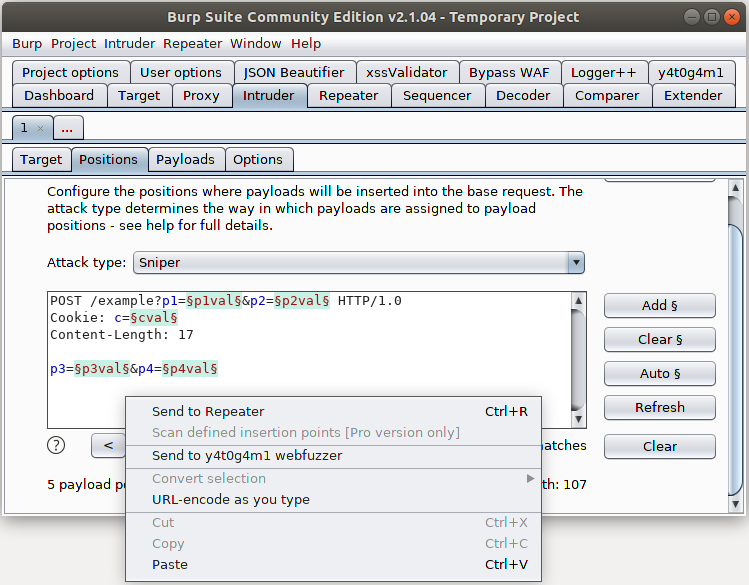
\includegraphics[width=0.8\textwidth,keepaspectratio=true]{images/send-base-request.png}
    \caption{Giao diện chính của chức năng Intruder}
    \label{fig:send-base-request-1}
\end{figure}
Giao diện chính của chức năng này gồm nhiều tab liền kề, mỗi tab được đánh số thứ tự, ứng với một \acrshort{http} request mẫu (base request) cần kiểm thử. Mỗi tab này gồm 4 tab phụ được mô tả như sau.
\begin{itemize}
    \item \textbf{Target} chứa thiết lập địa chỉ IP:port của ứng dụng web mục tiêu.
    \item \textbf{Positions} chứa những thiết lập của request mẫu cần kiểm thử, bao gồm các vị trí truyền tham số và kiểu tấn công.
    \item \textbf{Payloads} chứa các thiết lập liên quan đến tập payload kiểm thử. Tập payload này có thể được nhập từ tập tin trên máy, hoặc được sinh ra bằng một số phần mở rộng khác của Burp Suite, kèm theo các phương pháp tiền xử lí và encode payload thường dùng.
    \item \textbf{Options} chứa những thiết lập liên quan khác trong quá trình tấn công như thời gian chờ, các chuỗi và biểu thức chính quy để so trùng trên \acrshort{http} response trả về,...
\end{itemize}
Nhìn chung, chức năng này sử dụng cặp kí tự ``§'' để đánh dấu vị trí thay thế payload vào request mẫu để tạo thành requets kiểm thử, cụ thể việc sử dụng các danh sách payload và cách thức thay thế payload vào request mẫu như thế nào phụ thuộc vào kiểu tấn công của chức năng \texttt{Intruder}, gồm có \texttt{Sniper, Battering ram, Pitchfork} và \texttt{Cluster bomb}. Kiểu tấn công chúng tôi thường sử dụng nhất trong quá trình fuzzing bằng chức năng này là \texttt{Sniper}. Kiểu tấn công này chèn lần lượt từng payload trong danh sách vào từng vị trí thay thế payload trong request mẫu, do đó tổng số request kiểm thử được hình thành bằng tích số lượng payload nhân với số vị trí chèn payload trong request mẫu. Chúng tôi định ra hướng phát triển ứng dụng webfuzzer, hiện thực lại gần như đầy đủ chức năng \texttt{Intruder}, sử dụng kiểu tấn công \texttt{Sniper} vì những khuyết điểm của ứng dụng Burp Suite như sau.
\begin{itemize}
    \item Việc kiểm thử một request mẫu với nhiều loại lỗ hổng khá phiền phức, người dùng phải lần lượt sao chép các cấu hinh kiểm thử cần thiết vào tab chứa request mẫu. Do đó, nhu cầu định ra một cấu hình kiểm thử mặc định rồi dùng để kiểm thử các request mẫu với nhiều lỗ hổng, cộng với một giao diện trực quan, thân thiện với người dùng hơn, là cần thiết.
    \item Burp Suite không tự động thực thi yêu cầu kiểm thử tiếp theo sau khi hoàn thành yêu cầu hiện tại. Do đó việc xây dựng một ứng dụng kiểm thử xoay quanh các yêu cầu kiểm thử là cần thiết. Việc này giúp quản lý và phân phối tài nguyên máy tính hợp lý hơn, người dùng có thể kiểm soát một lúc có bao nhiêu yêu cầu kiểm thử đang thực thi, tự động thực thi những yêu cầu kiểm thử đã tạo trong thời gian nhàn rỗi, đồng thời cắt giảm thời gian thực hiện các thao tác lặp đi lặp lại của họ so với sử dụng Burp Suite.
    \item Ứng dụng có thể dễ dàng được triển khai ứng dụng kiểm thử ở các dịch vụ cung cấp máy chủ ảo hóa (virtual private service - \acrshort{vps}. Việc kiểm thử bằng Burp Suite trên máy tính cá nhân (đặc biệt là tính năng \texttt{Intruder}) tiêu tốn khá nhiều tài nguyên máy tính, cản trở công việc, dẫn đến nhu cầu tách riêng chức năng này để triển khai trên một máy chủ độc lập. Việc này cũng giúp tránh được nguy cơ địa chỉ IP của máy tính cá nhân bị block theo vùng địa lý hoặc bởi các chính sách kiểm soát lưu lượng truy cập bởi ứng dụng web mục tiêu do gửi quá nhiều request đến trong một khoảng thời gian ngắn, giúp người kỹ sư kịp thời định ra phương hướng khác để tiếp cận mục tiêu.
    \item Việc lưu trữ kết quả kiểm thử ở Burp Suite cần phải được làm bằng tay, dẫn đến nhu cầu cần có một cơ sở dữ liệu để lưu trữ, hệ thống hóa những điểm cuối ứng dụng web có lỗ hổng kèm theo bằng chứng khai thác được lỗi trong quá trình kiểm thử tự động. Việc xây dựng một cơ sở dữ liệu như webfuzzer cũng là tiền đề để mở rộng ứng dụng trên lĩnh vực do thám (reconnaissance) các ứng dụng web mục tiêu trong tương lai.
    \item Việc xây dựng một ứng dụng web để kiểm thử thay vì sử dụng Burp Suite ở máy tính cá nhân còn giải quyết được nhu cầu làm việc chung và chia sẻ dữ liệu kiểm thử của nhiều người trong cộng đồng, hay hẹp hơn là tổ chức, công ty, thay vì chỉ một cá nhân đơn lẻ. Nhiều người có thể trực tiếp đóng góp vào cơ sở dữ liệu và truy vấn thông tin bằng cách sử dụng ứng dụng webfuzzer thay vì Burp Suite ở máy tính cá nhân.
    \item Chỉ hiện thực chức năng so trùng trên chuỗi, biểu thức chính quy và kiểm tra thời gian phản hồi request của ứng dụng web mục tiêu, không hiện thực các chức năng nâng cao như kiểm thử đa luồng (multithread) và các hình thức encode đối với payload và \acrshort{url} vì payload đã được encode sẵn và thường chỉ thực hiện kiểm thử với 1 luồng, tránh trường hợp bị chặn bởi ứng dụng web mục tiêu do lưu lượng truy cập quá lớn.
\end{itemize}